\documentclass{scrreprt}

\usepackage{aligned-overset}
\usepackage{amsmath}
\usepackage{amssymb}
\usepackage{bm}
\usepackage[shortlabels]{enumitem}
\usepackage{hyperref}
\usepackage[utf8]{inputenc}
\usepackage{multicol}
\usepackage{mathtools}
\usepackage{physics}
\usepackage{tabularx}
\usepackage{titling}
\usepackage{fancyhdr}
\usepackage{xfrac}
\usepackage{pgfplots}

\pgfplotsset{compat = newest}
\usetikzlibrary{intersections}
\usetikzlibrary{patterns}
\usepgfplotslibrary{fillbetween}

\author{Karsten Lehmann}
\date{WiSe 2021/2022}
\title{Übungsblatt 01\\Analysis - Grundlegende Konzepte}

\setlength{\headheight}{26pt}
\pagestyle{fancy}
\fancyhf{}
\lhead{\thetitle}
\rhead{\theauthor}
\lfoot{\thedate}
\rfoot{Seite \thepage}

\begin{document}

\paragraph{1. Welche der folgenden Aussagen uber Element- und Teilmengenbeziehungen sind wahr?}

\begin{enumerate}[a)]
\item $a \in \qty{a, b}$

  \subparagraph{Lsg.} Diese Aussage ist wahr, das Element $a$ ist in der Menge
  mit den Elementen $a$ und $b$ enthalten.

\item $\qty{b, a, \emptyset} \subset \qty{a, b}$

  \subparagraph{Lsg.} Man sagt, dass eine Menge $N$ eine Teilmenge von der Menge
  $M$ ist, falls für jedes $n$ in $N$ gilt: $n \in M$.
  Die Leere Menge ($\emptyset$) ist zwar eine Teilmenge von $\qty{a, b}$ -
  allerdings kein Element aus $\qty{a, b}$.
  Somit ist diese Aussage falsch.

\item $\emptyset \in \emptyset$

  \subparagraph{Lsg.} Diese Aussage ist falsch.
  Die leere Menge ist zwar eine Teilmenge der leeren Menge, allerdings kein
  Element der leeren Menge.

\item $\emptyset \in \qty{a, b}$

  \subparagraph{Lsg.} Diese Aussage ist falsch.
  Die leere Menge ist zwar eine Teilmenge der Menge $\qty{a, b}$, allerdings kein
  Element der Menge $\qty{a, b}$.

\item $\emptyset \subset \qty{b} \in \qty\big{\qty{a}, \qty{b}}$

  \subparagraph{Lsg.} Diese Aussage ist wahr.
  Die leere Menge ist Teilmenge jeder anderen Menge und die Menge mit dem
  Element $b$ ist auch in $\qty\big{\qty{a}, \qty{b}}$ enthalten.

\item $\qty{a} \subset \qty\big{\qty{a}, \emptyset}$

  \subparagraph{Lsg.} Diese Aussage ist falsch, da das Element $a$ nicht in
  der Menge $\qty\big{\qty{a}, \emptyset}$ enthalten ist.
\end{enumerate}

\newpage
\paragraph{2. Klären Sie die Definition der Mengenoperationen $\cup$, $\cap$ und $\setminus$.
  Seien $A \coloneqq \qty{1, 2, 3, 4, 5}$ und $B \coloneqq \qty{2, 4, 6}$.
  Geben Sie die folgenden Mengen explizit an:}

\begin{enumerate}[a)]
\item $\qty(A \cup B) \setminus (A \cap B)$

  \subparagraph{Lsg.}
  \begin{center}
    \begin{tikzpicture}
      \node at (-0.2, 1.2) (label_a) {$A$};
      \node at (3.7, 1.2) (label_b) {$B$};
      \node at (1.75, -1.5) (label_ab) {$A \cap B$};
      \node[circle, draw, minimum size=2cm] at (1, 0) (set_a) {};
      \node[circle, draw, minimum size=2cm] at (2.5, 0) (set_b) {};
      \draw[->] (label_a) -- (set_a.center);
      \draw[->] (label_b) -- (set_b.center);
      \begin{scope}
        \clip (1, 0) circle (1cm) (2.5, 0) circle (1cm);
        \fill[even odd rule, pattern color=red, pattern=north west lines] (2.5, 0) circle (1cm) (1, 0) circle (1cm);
        \fill[even odd rule, pattern color=red, pattern=north west lines] (1, 0) circle (1cm) (2.5, 0) circle (1cm);
      \end{scope}
      \draw[->] (label_ab) -- (1.75, 0);
    \end{tikzpicture}
  \end{center}
  \begin{flalign*}
    \qty(A \cup B) &= \qty{1, 2, 3, 4, 5, 6} & \\
    \qty(A \cap B) &= \qty{2, 4} \\
    \qty(A \cup B) \setminus \qty(A \cap B) &= \qty{1, 3, 5, 6}
  \end{flalign*}

\item $B \setminus \qty\big(A \setminus \qty(A \cap B))$
  \subparagraph{Lsg.} $A \setminus \qty(A \cap B) = A \setminus B$

  $B \setminus \qty\big(A \setminus \qty(A \cap B)) = B = \qty{2, 4, 6}$

\item $\qty(A \setminus B) \cup \qty(B \setminus A)$

  \subparagraph{Lsg.}
  \begin{flalign*}
    A \setminus B &= \qty{1, 3, 5} & \\
    B \setminus A &= \qty{6} \\
    \qty(A \setminus B) \cup \qty(B \setminus A) &= \qty{1, 3, 5, 6}
  \end{flalign*}

\item $\qty\big(A \setminus \qty(A \cap B)) \cap B$

  \subparagraph{Lsg.}
  \begin{flalign*}
    A \setminus \qty(A \cap B) &= \qty{1, 3, 5} & \\
    B \cap \qty{1, 3, 5} &= \emptyset
  \end{flalign*}
\end{enumerate}

\end{document}